\documentclass[12pt]{article}

\usepackage[brazilian]{babel}
\usepackage[utf8]{inputenc}
\usepackage{graphicx}
\usepackage{mathtools}
\usepackage{amsthm}
\usepackage{thmtools,thm-restate}
\usepackage{amsfonts}
\usepackage{hyperref}
\usepackage[singlelinecheck=false]{caption}
\usepackage{enumitem}
\usepackage[justification=centering]{caption}
\usepackage{indentfirst}
\usepackage{algorithm}
\usepackage{algpseudocode}
\usepackage{listings}
\usepackage[x11names,rgb,table]{xcolor}
\usepackage{tikz}
\usepackage{hyperref}
\usepackage{subcaption}
\usepackage{booktabs}
\usepackage{linegoal}
\usepackage{geometry}
\usepackage{interval}
\usepackage[normalem]{ulem}
\usetikzlibrary{snakes,arrows,shapes}

\graphicspath{{imgs/}}

\makeatletter
\def\subsection{\@startsection{subsection}{3}%
  \z@{.5\linespacing\@plus.7\linespacing}{.1\linespacing}%
  {\normalfont}}
\makeatother

\DeclareMathOperator*{\argmin}{arg\,min}
\DeclareMathOperator*{\argmax}{arg\,max}
\DeclareMathOperator*{\Val}{\text{Val}}
\DeclareMathOperator*{\Ch}{\text{Ch}}
\DeclareMathOperator*{\Pa}{\text{Pa}}
\DeclareMathOperator*{\Sc}{\text{Sc}}
\newcommand{\ov}{\overline}
\newcommand{\tsup}{\textsuperscript}

\newcommand\defeq{\mathrel{\overset{\makebox[0pt]{\mbox{\normalfont\tiny\sffamily def}}}{=}}}

\newcommand{\algorithmautorefname}{Algorithm}
\algrenewcommand\algorithmicrequire{\textbf{Input}}
\algrenewcommand\algorithmicensure{\textbf{Output}}
\algnewcommand{\LineComment}[1]{\State\,\(\triangleright\) #1}

\captionsetup[table]{labelsep=space}

\theoremstyle{plain}

\newcounter{dummy-def}\numberwithin{dummy-def}{section}
\newtheorem{definition}[dummy-def]{Definition}
\newcounter{dummy-thm}\numberwithin{dummy-thm}{section}
\newtheorem{theorem}[dummy-thm]{Theorem}
\newcounter{dummy-prop}\numberwithin{dummy-prop}{section}
\newtheorem{proposition}[dummy-prop]{Proposition}
\newcounter{dummy-corollary}\numberwithin{dummy-corollary}{section}
\newtheorem{corollary}[dummy-corollary]{Corollary}
\newcounter{dummy-lemma}\numberwithin{dummy-lemma}{section}
\newtheorem{lemma}[dummy-lemma]{Lemma}
\newcounter{dummy-ex}\numberwithin{dummy-ex}{section}
\newtheorem{exercise}[dummy-ex]{Exercise}
\newcounter{dummy-eg}\numberwithin{dummy-eg}{section}
\newtheorem{example}[dummy-eg]{Example}

\numberwithin{equation}{section}

\newcommand{\set}[1]{\mathbf{#1}}
\newcommand{\pr}{\mathbb{P}}
\newcommand{\eps}{\varepsilon}
\newcommand{\ddspn}[2]{\frac{\partial#1}{\partial#2}}
\newcommand{\iddspn}[2]{\partial#1/\partial#2}
\renewcommand{\implies}{\Rightarrow}

\newcommand{\bigo}{\mathcal{O}}

\setlength{\parskip}{1em}

\lstset{frameround=fttt,
  frame=single,
  keepspaces=true,
	breaklines=true,
	keywordstyle=\bfseries,
	basicstyle=\footnotesize\ttfamily,
  language=Python
}

\newcommand{\code}[1]{\lstinline[mathescape=true]{#1}}
\newcommand{\mcode}[1]{\lstinline[mathescape]!#1!}

\newgeometry{margin=1in}
\title{%
  \textbf{Relatório MAC0318 EP6}\\
  \author{Renato Lui Geh --- NUSP\@: 8536030}
}
\date{}

\begin{document}

\maketitle

\section{Mapa}

O mapa criado para os testes foi gerado a partir de uma imagem $1024\times 720$. Na imagem, há
alguns polígonos rotacionados que criam os obstáculos. A área branca é desobstruída e as formas
pretas são os obstáculos.

\begin{figure}[h]
  \centering
\includegraphics[scale=0.4]{imgs/map.png}
  \caption{Mapa de polígonos onde a área branca indica desobstrução e formas pretas são
    obstáculos.}
\end{figure}

A classe \code{Map} representa o mapa de polígonos. Seu construtor aceita quatro argumentos: o
\textit{path} da imagem que representa o mapa, o tamanho do robô para dilatação, e o par $(b_x,
b_y)$ que parametrizam a discretização do mapa para o eixo $x$ e $y$ respectivamente.

Quando construído, \code{Map} gera dois mapas adicionais. O primeiro é a mesma imagem dilatada com
o tamanho do robô. Para isso foi usada a função \code{binary_dilation} do pacote
\code{scipy.ndimage.morphology}. A estrutura binária usada para a dilatação foi uma matriz $3\times
3$ com todos valores \code{true}. Desta forma, quando passada para a função de dilatação, será
feita uma dilatação quadrada de tamanho $d$.

O segundo mapa é a discretização aplicada ao mapa dilatado. Para isso, foi considerada uma
transformação de uma matriz $M(w, h)$ para $M(w/b_x, h/b_y)$, tal que toda região de pixel $b_x$
por $b_y$ é somada e normalizada entre 0 e 1 e em seguida transformada num só pixel $q=(q_x, q_y)$
cujo valor é o arredondamente da região original para o valor mais próximo 0 ou 1. Para isso, foi
usada a função \code{resize} e \code{threshold} do pacote \code{cv2}.

\section{Polígonos}

Para se detectar os polígonos no mapa, foi usada a função \code{findContours} do pacote \code{cv2}.
Esta função retorna os pontos de formas geométricas numa imagem. Estes pontos foram então juntados
para formar as linhas que definem o polígono. Por causa que imagens são representadas por uma
matriz, o espaço discreto faz com que haja imperfeições na detecção de formas. Então o número de
linhas detectadas foi maior do que se a detecção fosse ideal. No total foram geradas 1038 linhas a
partir desta função. A função também detecta a própria imagem como uma forma geométrica. Portanto,
além dos polígonos interiores, foi gerada também as bordas da imagem.

\begin{figure}[h]
  \centering
\includegraphics[scale=0.6]{imgs/contours.png}
  \caption{As linhas em cinza indicam a detecção das bordas das formas geométricas. Foram no total
    1038 linhas geradas.}
\end{figure}

\section{Configurações iniciais}

Foram feitos três testes com pontos iniciais e finais diferentes. Vamos denotar por $p=(p_x,p_y)$
e $q=(q_x,q_y)$ os pontos iniciais e finais respectivamente.

\begin{description}
  \item[Teste 1:] $p=(10, 10)$, $q=(1014, 710)$
  \item[Teste 2:] $p=(365, 61)$, $q=(365, 495)$
  \item[Teste 3:] $p=(61, 365)$, $q=(495, 365)$
  \item[Teste 4:] $p=(211, 555)$, $q=(588, 268)$
  \item[Teste 5:] $p=(555, 211)$, $q=(268, 588)$
\end{description}

O primeiro teste tenta cobrir um caminho por toda a image. O segundo tenta testar o quão bem o
algoritmo desvia do obstáculo. O terceiro é similar ao segundo, mas com os eixos trocados. O quarto
é o percurso mais fácil, mas que percorre um caminho entre vários polígonos. No quinto, os eixos
são trocados.

Para cada algoritmo, mostraremos uma imagem para cada teste feito, com o caminho feito pelo
algoritmo dado por pontos cinza claros e o caminho após linearização dado por linhas cinza escuras.

Vamos nos referir ao Teste $n$ como T.$n$. Então o Teste 3 será denotado por T.3.

\section{Frente de onda}

A função \code{wavefront} implementa o algoritmo, e a função \code{show_wavefront} cria uma imagem
para visualização do caminho. O algoritmo foi razoávelmente rápido e teve bons resultados.

\begin{figure}[H]
  \centering
\includegraphics[scale=0.4]{imgs/wavefront_path_1.png}
  \caption{Caminho da frente de onda para o T.1.}
\end{figure}

\begin{figure}[H]
  \centering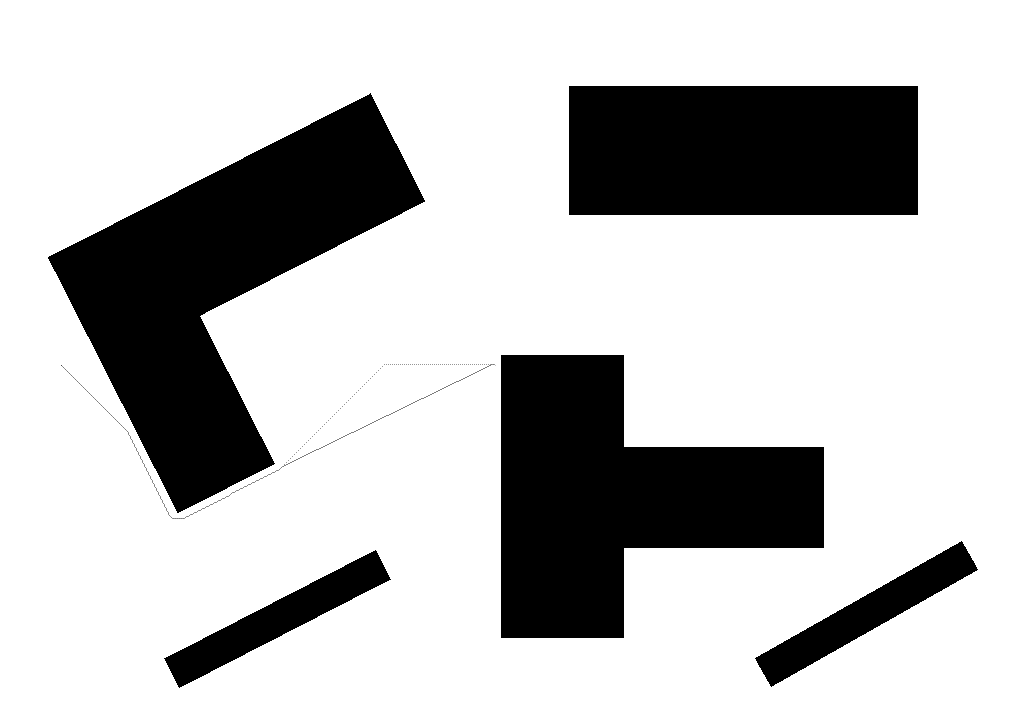
\includegraphics[scale=0.4]{imgs/wavefront_path_2.png}
  \caption{Caminho da frente de onda para o T.2.}
\end{figure}

\begin{figure}[H]
  \centering
\includegraphics[scale=0.4]{imgs/wavefront_path_3.png}
  \caption{Caminho da frente de onda para o T.3.}
\end{figure}

\begin{figure}[H]
  \centering
\includegraphics[scale=0.4]{imgs/wavefront_path_4.png}
  \caption{Caminho da frente de onda para o T.4.}
\end{figure}

\begin{figure}[H]
  \centering
\includegraphics[scale=0.4]{imgs/wavefront_path_5.png}
  \caption{Caminho da frente de onda para o T.5.}
\end{figure}

\section{Melhor escolha}

O algoritmo de melhor escolha foi implementado pela função \code{best_choice}, com a função
\code{show_best_choice} servindo para visualização do caminho.

Esta função toma um argumento adicional \code{mfunc}, que indica qual métrica usar: manhattan ou
euclideana. A escolha deste parâmetro mudou drásticamente tanto os resultados quanto o quão rápido
o algoritmo levou para computar os caminhos. A métrica Manhattan causou uma melhora muito
significativa no tempo de execucação. Para todos os caminhos, levou-se tanto tempo quanto ou muito
menos do que a frente de onda. No entanto, os resultados para o T.1 mostraram o problema que a
distância de Manhattan gera por não considerar as diagonais menos custosas.


\begin{figure}[H]
  \centering
\includegraphics[scale=0.4]{imgs/best_choice_manhattan_1.png}
  \caption{Caminho da melhor escolha com Manhattan para o T.1.}
\end{figure}

\begin{figure}[H]
  \centering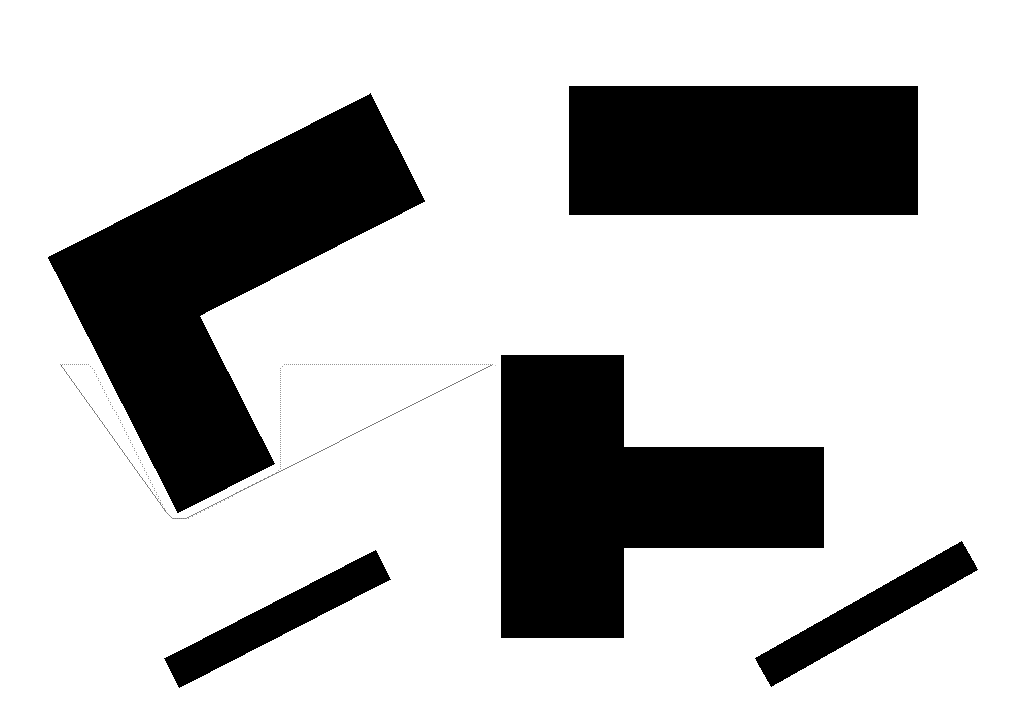
\includegraphics[scale=0.4]{imgs/best_choice_manhattan_2.png}
  \caption{Caminho da melhor escolha com Manhattan para o T.2.}
\end{figure}

\begin{figure}[H]
  \centering
\includegraphics[scale=0.4]{imgs/best_choice_manhattan_3.png}
  \caption{Caminho da melhor escolha com Manhattan para o T.3.}
\end{figure}

\begin{figure}[H]
  \centering
\includegraphics[scale=0.4]{imgs/best_choice_manhattan_4.png}
  \caption{Caminho da melhor escolha com Manhattan para o T.4.}
\end{figure}

\begin{figure}[H]
  \centering
\includegraphics[scale=0.4]{imgs/best_choice_manhattan_5.png}
  \caption{Caminho da melhor escolha com Manhattan para o T.5.}
\end{figure}

Para a distância euclideana, o tempo de execução foi muito maior que qualquer outro algoritmo.
Porém, foi a que gerou os melhores caminhos. Apesar disso, após linearização, os caminhos ficaram
praticamente iguais, mostrando que linearização pode melhorar muito uma solução subótima, levando
mais a pena buscar uma solução subótima mas rápida e depois pós-processar com linearização.

\begin{figure}[H]
  \centering
\includegraphics[scale=0.4]{imgs/best_choice_euclidean_1.png}
  \caption{Caminho da melhor escolha com Euclideana para o T.1.}
\end{figure}

\begin{figure}[H]
  \centering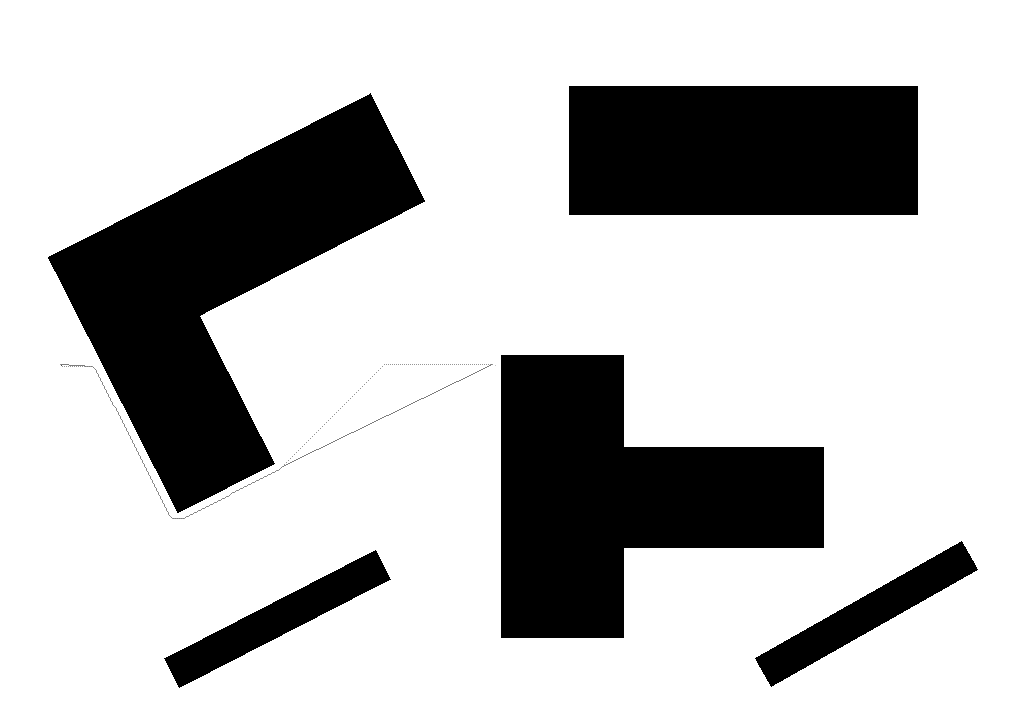
\includegraphics[scale=0.4]{imgs/best_choice_euclidean_2.png}
  \caption{Caminho da melhor escolha com Euclideana para o T.2.}
\end{figure}

\begin{figure}[H]
  \centering
\includegraphics[scale=0.4]{imgs/best_choice_euclidean_3.png}
  \caption{Caminho da melhor escolha com Euclideana para o T.3.}
\end{figure}

\begin{figure}[H]
  \centering
\includegraphics[scale=0.4]{imgs/best_choice_euclidean_4.png}
  \caption{Caminho da melhor escolha com Euclideana para o T.4.}
\end{figure}

\begin{figure}[H]
  \centering
\includegraphics[scale=0.4]{imgs/best_choice_euclidean_5.png}
  \caption{Caminho da melhor escolha com Euclideana para o T.5.}
\end{figure}

\section{Campo potencial}

O algoritmo de campo potencial foi implementado pela função \code{potential}, junto com seu
equivalente para visualização \code{show_potential_field}. O algoritmo aceita como parâmetros:
$k_a$, a constante de atração; $k_r$, a constante de repulsão; $\alpha$, a taxa de atualização;
$\rho$, a distância máxima de influência; $\epsilon$, o critério de convergência; $p$, o ponto
inicial e $q$ o ponto final. Para os testes, foram usados os seguintes valores para os parâmetros:

\begin{description}
  \item[$k_a$]$=0.1$
  \item[$k_r$]$=1000$
  \item[$\alpha$]$=0.1$
  \item[$\rho$]$=200$
  \item[$\eps$]$=1.0$
\end{description}

Em questão de tempo de execução, o campo potencial foi o mais rápido na maior parte dos casos. O
algoritmo de campo potencial foi o único a não conseguir completar todos os testes, já que não
completou o T.1. Foi implementado um jeito de tentar sair do ótimo local, mas mesmo assim, em
alguns pontos o algoritmo ainda ficava preso, então foi decidido não deixar no código final. Mesmo
assim, deixei o código no Apêndice.

As trajetórias do campo potencial, como era de se esperar, foram as mais ``suaves''. Mesmo assim,
após linearização ficaram parecidas com os outros algoritmos. Em alguns casos, a linearização teve
problema com os pontos, e acabaram causando linearizações erradas. Como foi implementada a versão
usando a força, não seria necessária a linearização.

Como o campo potencial não consegue completar o T.1, foi omitido o teste e mostrado os restantes.

\begin{figure}[H]
  \centering
\includegraphics[scale=0.4]{imgs/potential_field_1.png}
  \caption{Caminho do campo potencial para o T.2.}
\end{figure}

\begin{figure}[H]
  \centering
\includegraphics[scale=0.4]{imgs/potential_field_2.png}
  \caption{Caminho do campo potencial para o T.3.}
\end{figure}

\begin{figure}[H]
  \centering
\includegraphics[scale=0.4]{imgs/potential_field_3.png}
  \caption{Caminho do campo potencial para o T.4.}
\end{figure}

\begin{figure}[H]
  \centering
\includegraphics[scale=0.4]{imgs/potential_field_4.png}
  \caption{Caminho do campo potencial para o T.5.}
\end{figure}

\section{Apêndice}

Código para tentativa de sair de um ótimo local. A ideia era tomar os vetores ortogonais (no caso
normalizamos, então temos os ortonormais) ao vetor força. Existem dois, um que segue uma direção
parecida à força de repulsão e outra que está na direção contrária da repulsão. Tome por $u$ e $v$
os vetores ortonormais ao vetor força $f$, e chame de $f_r$ a força de repulsão. Então queremos o
vetor força

\begin{equation*}
  \argmin_{p\in\{u,v\}}\{||u-f_r||, ||v-f_r||\},
\end{equation*}

já que não queremos ir em direção a obstrução. Após tomarmos $p$ deste mínimo, aplicamos uma
constante nele e somamos à posição atual.  O problema desta solução é achar uma constante grande o
suficiente para tirar o algoritmo do ótimo local e ao mesmo tempo não estourar as
coordenadas.\newpage

\begin{lstlisting}[language=Python]
def potential(self, k_att, k_rep, alpha, rho, eps, sx, sy, tx, ty):
  C = []
  P = [(sx, sy)]
  for c in self.L:
    C.append((np.array([c[0], c[1]]), np.array([c[2], c[3]])))
  p = np.array([sx, sy])
  g = np.array([tx, ty])
  f = np.inf
  last = p
  n = linalg.norm(f)
  d = linalg.norm(p-g)
  while n > eps or d > 50.0:
    att, rep = self.f_att(p, g, k_att), self.f_rep(k_rep, rho, p, C)
    f = att+rep
    p = p+alpha*f
    if not np.array_equal(last.astype(int), p.astype(int)) and \
       (0 <= p[0] <= self.w and 0 <= p[1] <= self.h):
      print(p, self.orig_pos(p))
      P.append((p[0], p[1]))
      last = np.copy(p)
    n = linalg.norm(f)
    d = linalg.norm(p-g)
    if n <= 2 and d > 50.0:
      # Give it a push. Find orthogonal vector and push in this direction.
      r = np.random.randn(2)
      r -= r.dot(f)*f / np.linalg.norm(r)**2
      r /= np.linalg.norm(r)
      dr, ds = np.linalg.norm(rep-r), np.linalg.norm(rep+r)
      df = -r if dr < ds else r
      p = p+20*df+alpha*f
      n = linalg.norm(f)
  P.append(g)
  P = list(np.unique(P, axis=0).astype(int))
  return P
\end{lstlisting}

\end{document}
